\begin{figure}[H]
\caption{Clasificación de los programas maliciosos}
\centering
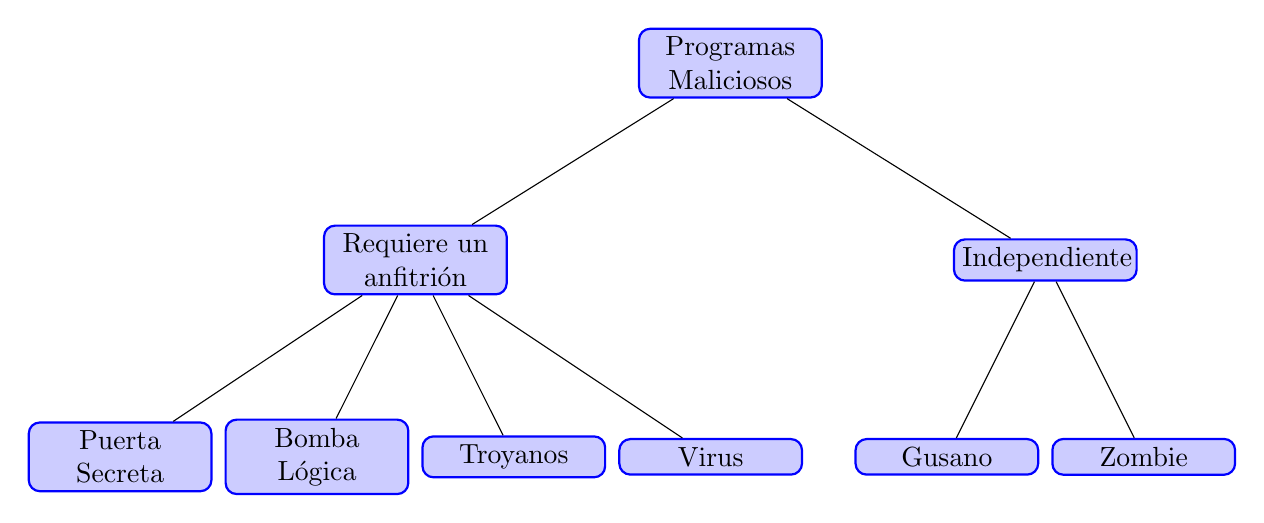
\begin{tikzpicture}[auto, 
       every node/.style={draw=blue, thick, fill=blue!20,
             text width=6em, text badly centered,inner sep=3pt, rounded corners}, 
       level 1/.style={sibling distance=80mm, level distance=2.5cm},
       level 2/.style={sibling distance=25mm, level distance=2.5cm}]
\node[draw](z){Programas Maliciosos}
    child{ 
        node {Requiere un anfitrión}
        child{
            node {Puerta Secreta} }
        child{
            node {Bomba Lógica} }
        child{
            node {Troyanos} }
        child{
            node {Virus} }
    } 
    child{ 
        node {Independiente}
        child{
            node {Gusano} }
        child{
            node {Zombie} }
    };
\end{tikzpicture}
\label{fig:malware}
\end{figure}
